\chapter{Introduction}

In this first chapter we want to familiarize the reader with the scientific
background of our work and its motivation. We hope to clarify what basic
questions the discipline of ultracold atom experiments tries to solve. In a
second part we want to elaborate on the concepts of localized optical
potential dynamcis and summarize the related work reported by the community.

\subsubsection{Background}

Many body quantum systems studied inter alia in condensed matter physics are
experimentally challenging to access as any interactions can destroy the
carefully prepared quantum states. As a way forward, experiments with
ultracold atoms in optical lattices give us a highly controllable
environment, permitting us to simulate and explore quantum effects and expand
our current understanding of quantum mechanics and statistical physics
\cite{Gross2017}.

\begin{figure}[ht]
  \centering
  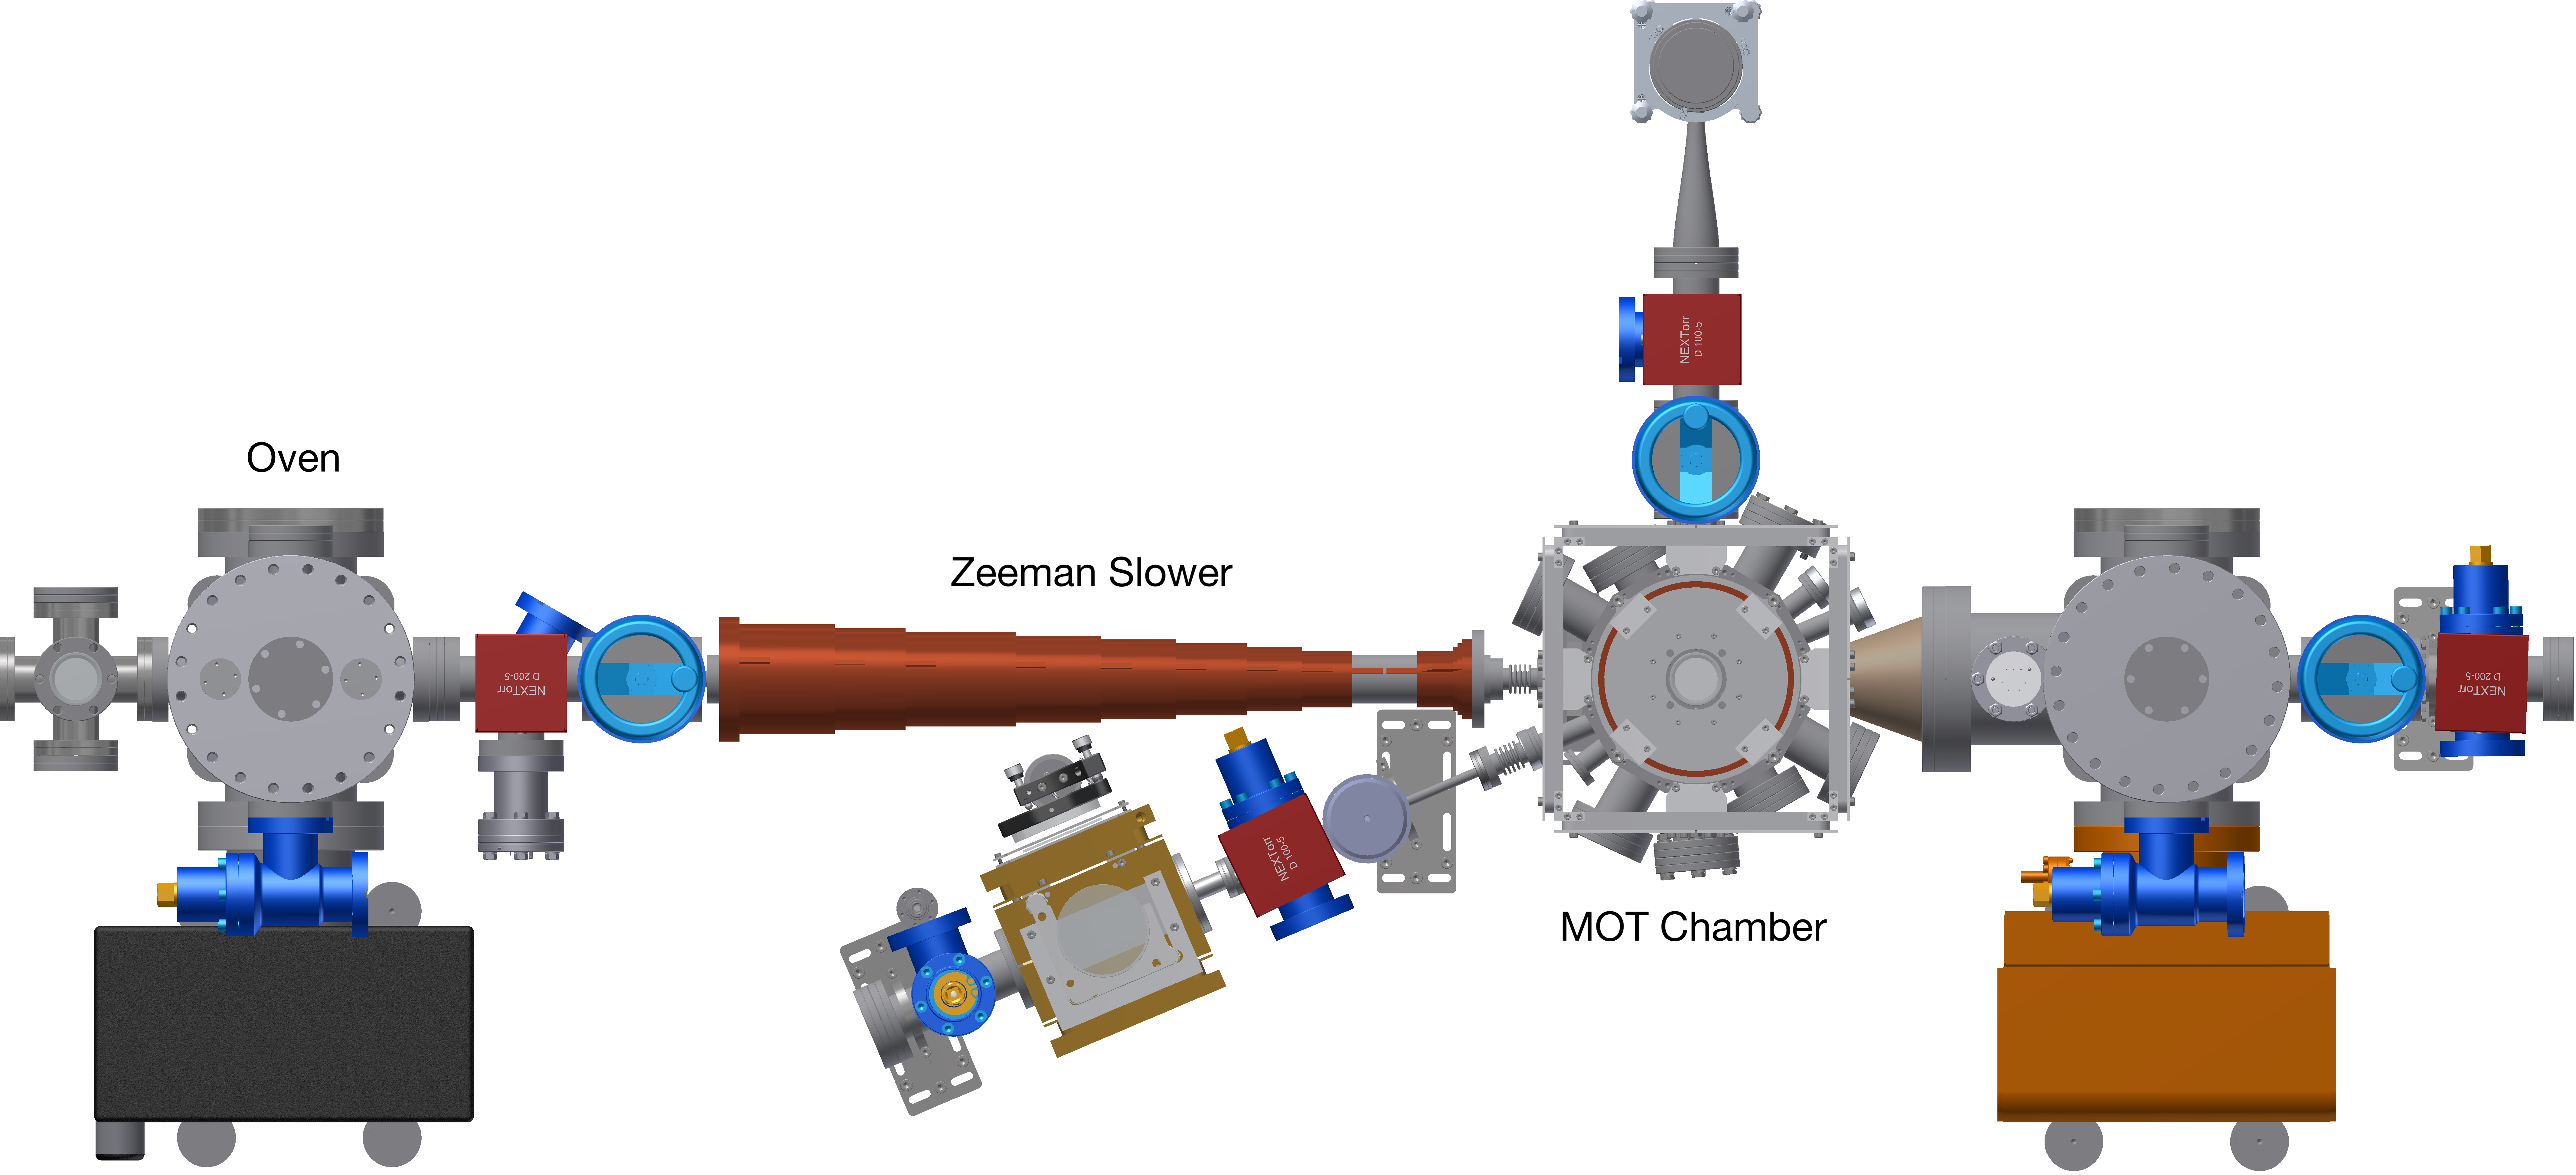
\includegraphics[width=\textwidth]{\mediadir{setup/apparatus.png}}
  \captionsetup{width=.9\textwidth}
  \caption{Vacuum setup of the Caesium experiment. On the left-hand
  side an oven heats up atoms from the bottom. An ensemble of atoms with the
  correct momentum direction move towards the pipe on the right. The Zeeman
  slower in the middle creates a magnetic gradient such that the atoms are in
  resonance with cooling laser antiparallel to their flight direction.
  Finally the atoms are loaded into the optical lattice inside the \gls{mot}
  chamber where the actual experiments are then conducted.}
  \label{fig:ultracold_atoms_setup}
\end{figure}

The apparatus used for ultracold atoms experiments is a vacuum system that
cools down neutral atoms to temperatures of below micro Kelvin and loads them
into an optical lattice. In \Cref{fig:ultracold_atoms_setup} the major
components of the vacuum apparatus of the Caesium experiment are depicted.
The oven on the left-hand side heats up the atoms. Atoms with the correct
momentum direction move to the right. The Zeeman slower in the middle creates
a magnetic field gradient such that the atoms are always in resonance with
the cooling laser antiparallel to the momentum direction. In the \gls{mot}
chamber atoms are further cooled to target temperature and loaded into the
optical lattice where experimental sequences can take place
\cite{Lewenstein2007}.

\begin{figure}[ht]
  \centering
  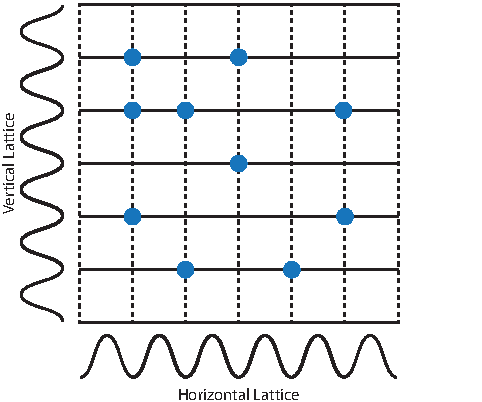
\includegraphics[width=.6\textwidth]{\mediadir{diagram/optical-lattice.pdf}}
  \captionsetup{width=.9\textwidth}
  \caption{Two dimensional optical lattice for an ultracold atom experiment.
    The atoms (blue) sit on their respective lattice site (rectangular grid
    nodes) created by the superposition of two periodic potentials (outside).}
  \label{fig:optical_lattice}
\end{figure}

In \Cref{fig:optical_lattice} a two dimensional optical lattice used in
ultracold atoms experiments is presented. The atoms (blue) sit on their
respective lattice site (rectangular grid nodes) which are created by the
superposition of two light fields (left and bottom). In such periodic
structures the atomic wave functions already show amazing similarity to the
electron wave functions theorized in solids like the energy band structure.
However one can think of many different variations to the simple lattice
structure depicted in \Cref{fig:optical_lattice} like for example hexagonal
lattice structures or superlattices, i.e. lattices with lattice
substructure.

\subsubsection{Motivation}

As a matter of fact the design and engineering of the respective lattice
structure and dynamic is of crucial importance to uncover new physics in
ultracold atoms experiments. Beside of the changes of the global lattice
structure we can also think of local changes. With reference of our simple
lattice in \Cref{fig:optical_lattice} we can think of two simple alterations
which we illustrated in \Cref{fig:local_optical_lattice}.

\begin{figure}[ht]
  \centering
  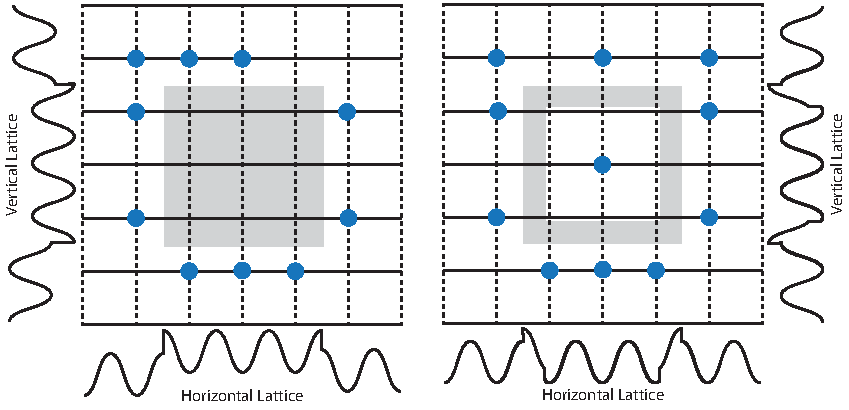
\includegraphics[width=\textwidth]{\mediadir{diagram/local-optical-lattice.pdf}}
  \captionsetup{width=.9\textwidth}
  \caption{Two dimensional optical lattices for an ultracold atom experiment
    with local alterations. One the left we have a local potential step that
    pushes atoms with lower energy away wheras on the right we created a
    local potential barrier that entraps an atom.}
  \label{fig:local_optical_lattice}
\end{figure}

In the left embodiment we applied a two dimensional potential well to the
center of the lattice. If the potential well is sufficient large compared to
the energies of the surrounding atoms it will push the atoms away which can
also be thought of as a impurity inside a solids lattice structure.

In the right embodiment we apply two small potential wells to each potential
dimension yielding a potential barrier that can entrap atoms. Physical
applications of such barrier could be used to further study thermodynamic
exchange processes or if applied dynamically could be use to sweep atom
states.

Anyway there are of course many more possibilites to change the local
topology of optical lattice structures.

\subsubsection{Related work}

Local manipulations of atoms inside optical lattices have been known for some
time in the manifestatiion of optical tweezers that allow trapping, stacking
and sorting of particles \cite{Tadmor2004}. Yet, only recently attempts to
interact with local particle clusters through high-precision time-averaged
optical potentials have been reported \cite{Roy2016}.

The key concept to create local optical potentials is similar to the
principle with what cathode ray tube screens operate. The idea is to
consecutively illuminate a finite point set that covers the desired space.
A complete passthrough of the finite point set has to occur on a time scale
short compared to the time scale of the observed processes such that over
average the passthrough yields an effective potential in the observed
process.

In comparison to the state of art which uses mechanical mirror arrays for
beam deflection \cite{Roy2016} our approach exercises acousto-optical
deflection by \gls{aod}. In the following we continue on the ground work
laid out in \cite{Hertlein2017} which provided us with an optical setup for
single-site manipulation using \gls{aod} as well as the discussion of
aperture limited gaussian beam propagation.

\subsubsection{Outline}

We will start of with the theoretical foundation of optical lattice
potentials and give more details on how the lattice potential alters under
an additional potential well. From there on we will estimate the required
time scale set by hopping frequency of atoms between lattice sites. After
a short introduction to direct digital signal synthesis we will calculate
if and how the used \gls{dds} met the previously found demands. That in place
we can continue with an overview of our experimental setup and results. The
experiments separate in a part concerning the radio electronics, a part
dedicated to the intensity transmission subject to the \gls{rf} signal and
a final part where we attempt to minimize the intensity transmission
variance.
